\begingroup
	\pgfdeclarelayer{background layer}
	\pgfsetlayers{background layer,main}
	\tikzstyle{zero}=[circle,draw=black,fill=white,inner sep=0pt,minimum size=3.5mm]
	\tikzstyle{one}=[circle,draw=black,fill=black,inner sep=0pt,minimum size=3.5mm]
	\tikzstyle{two}=[circle,draw=black,fill=gray,inner sep=0pt,minimum size=3.5mm]
		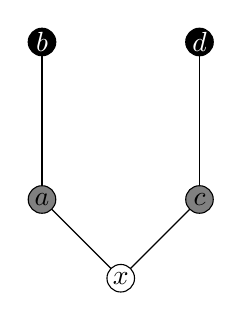
\begin{tikzpicture}
			\node [white] at (-1,1) [one] {$b$};
			\node at (1,-1) [two] {$c$};
			\node [white] at (1,1) [one] {$d$};
			\node at (-1,-1) [two] {$a$};
			\node at (0,-2)	[zero] {$x$};		
			\begin{pgfonlayer}{background layer}				
				\draw (-1,1)--(-1,-1);
				\draw (1,1)--(1,-1);
				\draw (0,-2)--(1,-1);
				\draw (0,-2)--(-1,-1);					
			\end{pgfonlayer}			
		\end{tikzpicture}
	%\label{fig:hasse_graded_poset_min}	
\endgroup